\documentclass[border=10pt]{standalone}

\usepackage{tikz}
\usetikzlibrary{shapes,arrows}

\begin{document}

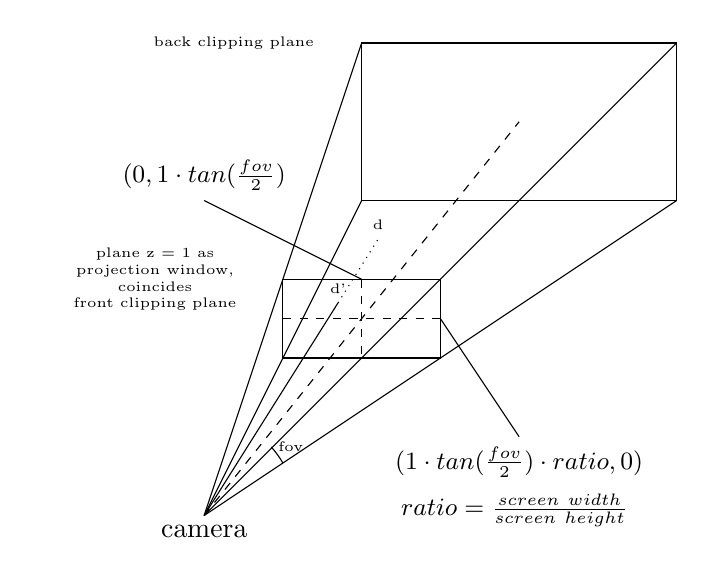
\begin{tikzpicture}
 
    \coordinate (o) at ( 0,  0);
    \coordinate (NA) at ( 1,  3);
    \coordinate (NB) at ( 3,  3);
    \coordinate (NC) at ( 3,  2);
    \coordinate (ND) at ( 1,  2);
    
    \coordinate (Nt) at ( 2,  3);
    \coordinate (Nb) at ( 2,  2);
    \coordinate (Nl) at ( 1,  2.5);
    \coordinate (Nr) at ( 3,  2.5);
    
    \coordinate (NO) at ( 2,  2.5);
    
    \coordinate (d') at ( 1.7,  2.7);
    \coordinate (dx') at ( 1.7,  2.5);
    \coordinate (dy') at (   2,  2.7);
    \coordinate (d) at ( 2.21,  3.51);
    
    \coordinate (FA) at ( 2,  6);
    \coordinate (FB) at ( 6,  6);
    \coordinate (FC) at ( 6,  4);
    \coordinate (FD) at ( 2,  4);
    \coordinate (FO) at ( 4,  5);
    
    \draw (NA) rectangle (NC);
    \draw (FA) rectangle (FC);
    
    \draw (o) -- (FA);
    \draw (o) -- (FB);
    \draw (o) -- (FC);
    \draw (o) -- (FD);
    
    \draw [dashed] (o) -- (FO);
    \draw [dashed] (Nt) -- (Nb);
    \draw [dashed] (Nl) -- (Nr);
    
    \draw (o) -- (d');
    \draw [dotted] (d') -- (d);
    
    \node [below] at (o) {camera};
    \node [above, font=\tiny] at (d) {d};
    \node [above, font=\tiny] at (d') {d'};
    
    \node [text width=3cm, text centered, font=\tiny, left] at (NA) {plane z = 1 as\\projection window,\\coincides\\front clipping plane};
    \node [text width=3cm, text centered, font=\tiny, left] at (FA) {back clipping plane};
    
    \draw (Nt) -- (0, 4) node [above, font=\small] {$(0, 1 \cdot tan(\frac{fov}{2})$};
    \draw (Nr) -- (4, 1) node [below, font=\small] {$(1 \cdot tan(\frac{fov}{2}) \cdot ratio , 0)$};
    \node [text width = 3cm, below, font=\small] at (4, 0.4) {$ratio = \frac{screen\ width}{screen\ height}$};
    
    \draw (1, 2/3) arc [x radius=1.2, y radius=1.2, start angle=30, end angle=42];
    \node [above, font=\tiny] at (1.1, 0.69) {fov};
    
\end{tikzpicture}
\end{document}

    
